\hypertarget{ux9065ux63a7ux8f6cux5411}{%
\subsection{遥控转向}\label{ux9065ux63a7ux8f6cux5411}}

前面我们讲了如何遥控小车前进后退,以及使用传感器自动停止。但是,细心的童鞋可能发现了,这个小车不能拐弯,只能走直线,这样就少了很多乐趣。

为啥这个小车不能拐弯呢?因为要拐弯,需要控制前轮转向,或者控制两个轮子的转速,通过转速差实现转向。

控制前轮转向比较麻烦,而控制两个轮子的转速比较简单。我们把小车升级一下,用两个马达搭建一个坦克:

 
 \begin{figure}[htp]
	\centering
	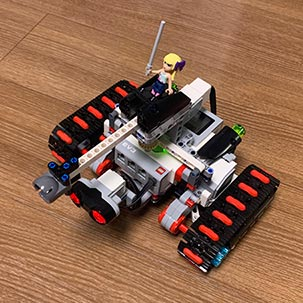
\includegraphics[width=0.6\linewidth]{fig/1346727531511874l.png}
\end{figure}


这个坦克除了有两个马达控制左右轮之外,还有一个马达控制炮台转动。

通过两个马达控制转速实现转向时,我们只要根据轮子的直径、轮距,就可以计算出在给定速度和转向角度时两个马达的转速,计算过程如下:

(此处为一堆乱码)

因为计算过程比较繁琐,所以 EV3
直接提供了一个\texttt{DriveBase}类自动计算并设定两个马达的转速。我们用一个\texttt{Driver}类包装一下,实现如下:

\begin{pythoncode}
class Driver():
    def __init__(self, leftMotor, rightMotor, diameter, axle):
        self.driver = DriveBase(leftMotor, rightMotor, diameter, axle)
        self.x = 0
        self.y = 0
        self.speed = 0
        self.steering = 0

    def drive(self, speed, steering):
        self.speed = speed
        self.steering = steering
        if self.speed == 0:
            self.driver.stop()
        else:
            self.driver.drive(self.speed, self.steering)
\end{pythoncode}

在 Robot 类中,我们需要传入必要的参数以构造\texttt{Driver}:

\begin{pythoncode}
class Robot():
    def __init__(self, leftMotor, rightMotor, diameter, axle, maxSpeed=300, maxSteering=180):
        self.driver = Driver(leftMotor, rightMotor, diameter, axle)
        self.speedStep = 32767 // maxSpeed
        self.steeringStep = 32767 // maxSteering
        ...

    def drive(self, x, y):
        speed = -y // self.speedStep
        steering = x // self.steeringStep
        self.driver.drive(speed, steering)
\end{pythoncode}

当我们从摇杆接收到\texttt{x}、\texttt{y}坐标后,先转换成速度和转向角度,再调用\texttt{DriveBase.drive(speed,\ steering)}方法,即可按指定速度和角度转向。注意到\texttt{x}、\texttt{y}坐标先处理成以\texttt{(0,\ 0)}为原点的坐标,以便于计算。

最后来看看实际效果:

\hypertarget{ux53c2ux8003ux6e90ux7801}{%
\subsubsection{参考源码}\label{ux53c2ux8003ux6e90ux7801}}

\href{https://github.com/michaelliao/learn-python3/tree/master/samples/micropython/tank}{tank}

